\section{图的存储结构}

\begin{figure}[H]
	\centering
	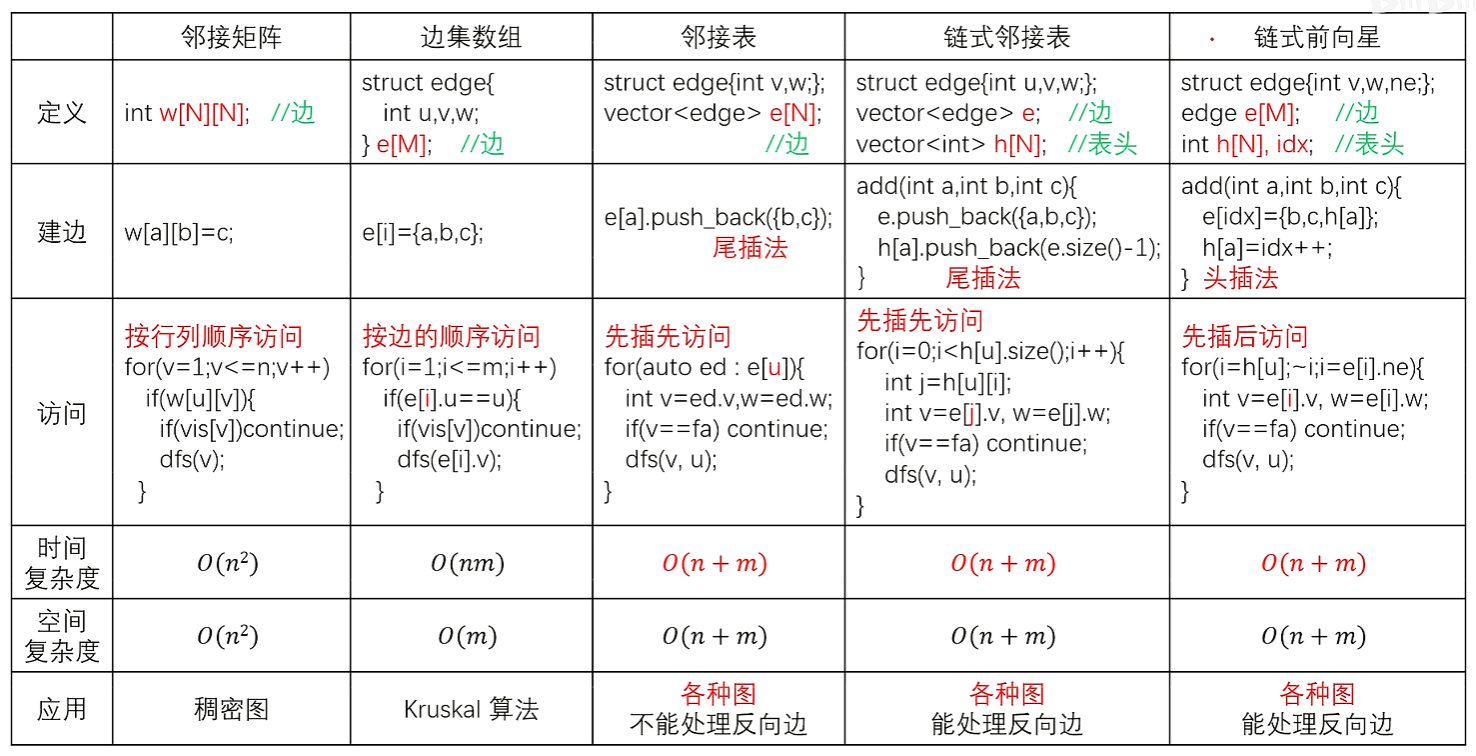
\includegraphics[width=0.99\linewidth]{figure/cunchujiegou}
	\caption{图的存储}
	\label{fig:cunchujiegou}
\end{figure}


\subsection{邻接矩阵}

\begin{lstlisting}[language=c++]
///////邻接矩阵 示例 
#include <bits/stdc++.h>
using namespace std;
const int N=1010,M=1010;
int n,m,a,b,c;
int w[N][N];//边权 
int vis[N];
void dfs(int u){
	vis[u]=true;
	for(int v=1;v<=n;v++)
	if(w[u][v]){
		printf("%d,%d,%d\n",u,v,w[u][v]);
		if(vis[v]) continue;
		dfs(v);
	}
}
int main(){
	cin>>n>>m;
	for(int i=1;i<=m;i++){
		cin>>a>>b>>c;
		w[a][b]=c; 
		// w[b][a]=c;
	}
	dfs(1);
	return 0;
}
\end{lstlisting}

\begin{figure}[H]
	\centering
	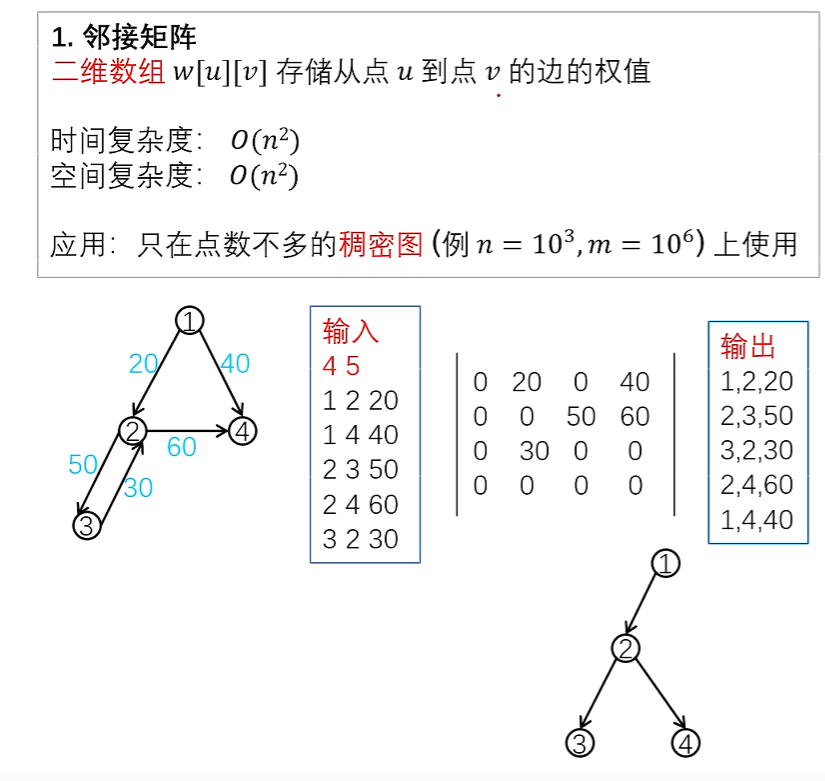
\includegraphics[width=0.99\linewidth]{figure/linjiejuzhen}
	\caption{邻接矩阵介绍}
	\label{fig:linjiejuzhen}
\end{figure}
